\chapter{Descripción del proyecto}
En este capítulo se describe cómo funciona el motor en esencia, es decir, sin entrar en la implementación del mismo. Esta idea general no depende del lenguaje de programación.

Hay un apartado que describe al motor y sus capacidades, y otro apartado que muestra el diseño actual de la aplicación y expone otras ideas que se pueden llevar a cabo.

\section{Qué es Historias del Laberinto (Descripción)}
Historias del Laberinto es una aplicación que funciona como \textbf{intérprete de videojuegos}. Los posibles nombres con los que se identifica al motor en este trabajo son motor, intérprete, aplicación o proyecto.

Esta aplicación permite a un usuario reproducir un videojuego definido en un formato predefinido. Este formato permite abstraer de toda la capa programática a un diseñador.
De momento solo es capaz de reproducir videojuegos, no es capaz de crearlos, aunque en una futura versión probablemente se desarrolle esta opción.

Se ha referido antes al proyecto también como un motor de videojuegos, que se puede definir de esta manera:
\begin{quote}
	\small Un motor de videojuego es un término que hace referencia a una serie de librerías de programación que permiten el diseño, la creación y la representación de un videojuego. \cite{Alberto_Carrasco}
\end{quote}

En el caso de este trabajo, el proyecto no es una serie de librerías sino que es directamente una aplicación. De esta manera, se puede abstraer a un creador del videojuego de la programación directa de un juego.

Otros motores de videojuego que ahora están en el mercado y tienen una funcionalidad similar son Unreal Engine\cite{unrealEngineHomepage} o Unity\cite{unity3dHomepage}. Estos motores permiten crear videojuegos con una capacidad genérica muy potente, pero en muchos casos necesitan que el diseñador tenga conocimientos de diseño 3D, programación y matemáticas. No se ha conseguido llegar al nivel de estos motores, porque supondría un reto muy grande para el ámbito de un trabajo de fin de grado.

\begin{figure}[h]
	\caption{Logo del motor Unreal engine}
	\centering
	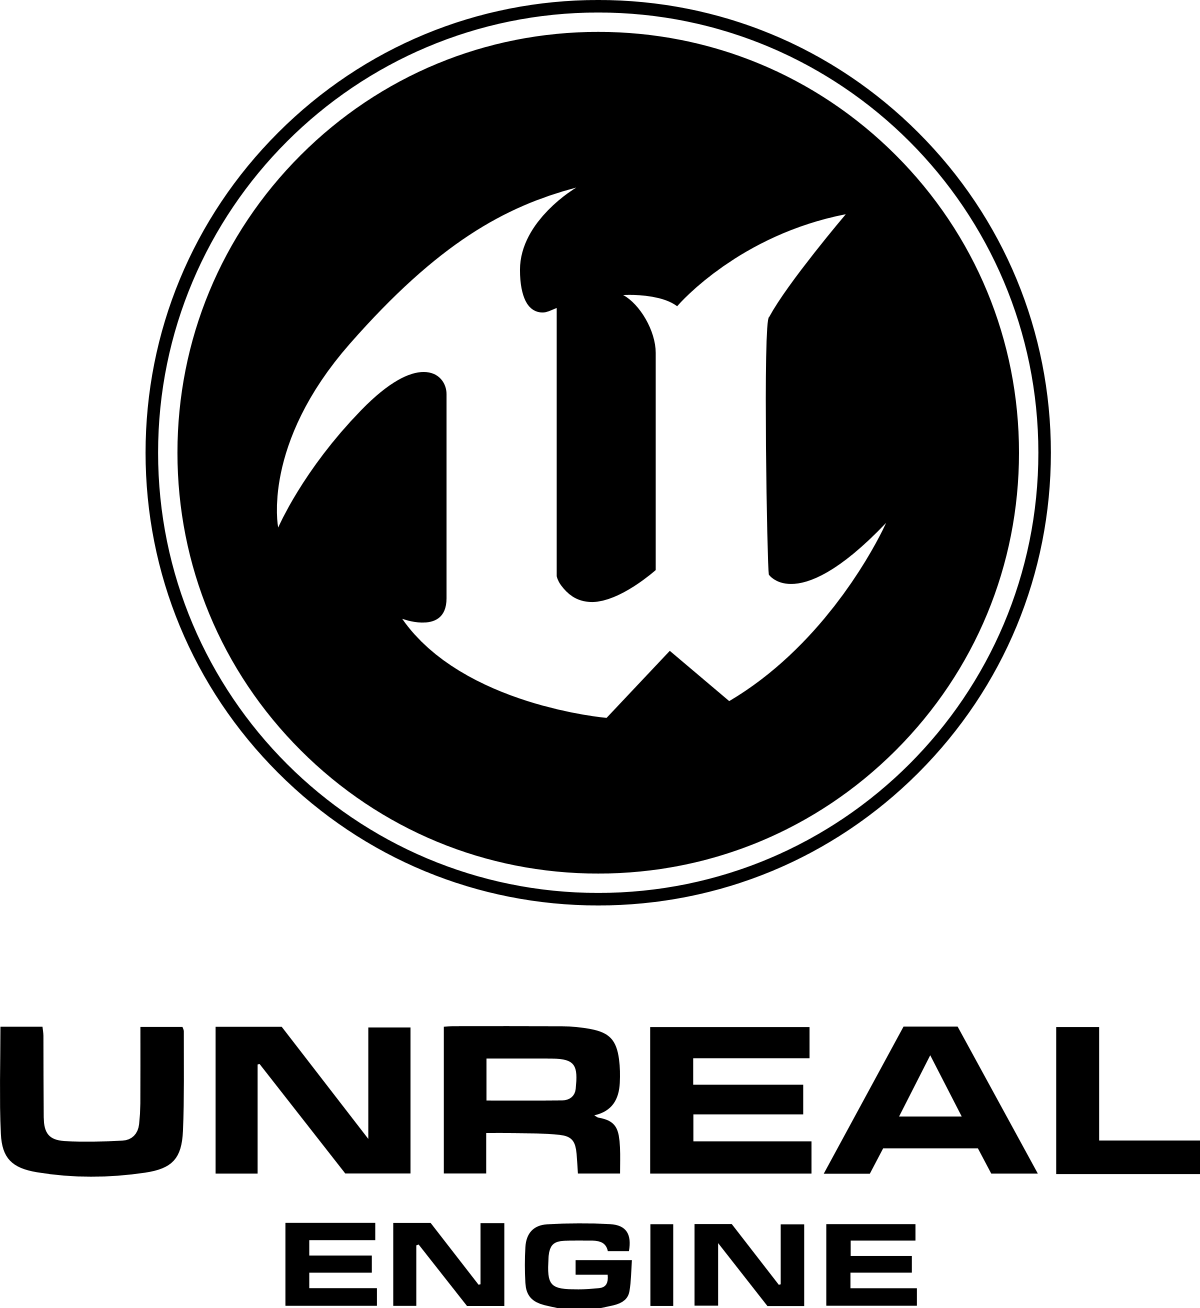
\includegraphics[width=0.3\textwidth]{include/unrealEngineLogo.png}
\end{figure}

\subsection{Qué tipo de videojuegos se pueden crear}
El interprete está orientado a reproducir juegos en los que el jugador tiene que escapar de una mazmorra. Para ello, el jugador debe reunir objetos como llaves para abrir puertas, esquivar trampas, resolver rompecabezas, luchar contra monstruos, usar pociones y llegar a una habitación final.
Algunos ejemplos de juegos parecidos a los que está orientado el motor son ''Dragones y Mazmorras'' o los libros de ''elige tu propia aventura''.

Aunque el motor esté desarrollado con una fuerte influencia por este tipo de juegos, no está limitado a ellos, cualquier creador pueda ir más allá de este concepto o incluso cambiarlo radicalmente usando las herramientas genéricas de las que dispone el motor. El límite lo pone la imaginación del usuario.

\subsection{Dónde se podrá usar el motor}
De momento sólo está disponible para dispositivos que soporten el sistema operativo iOS, es decir, solo para dispositivos portables de Apple, como un iPhone o un iPad.
Tampoco hay planes actuales de mover el motor a otra plataforma, pero es posible implementar el motor en otros sistemas y lenguajes de programación.

Con todas estas dudas resueltas ya solo queda mostrar las funciones de las que dispone el motor.

\subsection{Qué es capaz de hacer el motor}
El proyecto anterior se considera un punto de partida para muchos conceptos que se querían llevar a cabo para el nuevo motor. Por ello, se escogieron ciertas funcionalidades comunes que permitieran representar al videojuego original, separandolas en pequeñas piezas: mostrar un diálogo, iniciar un combate...
De esta manera nacen los \textbf{eventos}.

El juego original también contaba con una serie de jugadores con los que podía interactuar el usuario, salas en las que se desarrollaba la historia, un sistema de movimiento en forma de cuadrícula... Todos estos aspectos se han traducido al motor de manera que sean lo más fieles posibles al juego original.

A continuación, se describen por partes las funcionalidades que tiene el motor. De momento no se entra en las especificaciones propias de la implementación, pero aparecerá el diseño llevado a cabo en la sección \ref{designSection}, y cómo se ha implementado en el capítulo \ref{applicationImplementation}.

\subsection{Eventos}
Un evento representa una acción atómica que puede realizar el motor. Estas acciones se consideran básicas en el ámbito de una aventura, como escoger una opción o mostrar un diálogo; aunque requieran de más trabajo a la hora de programarlas.

Los eventos están pensados para unirse entre ellos, de manera que se puedan mezclar entre sí varias acciones básicas para formar una cadena de eventos. Por ello, cualquiera de ellos son intercambiables, intercalables y no pueden tener dependencias entre sí.
Además, siempre se ejecutan de forma lineal, siguiendo un orden predefinido por el creador del juego.

El centro de toda la potencia del motor reside en los eventos, ya que son un mecanismo genérico y preciso de ejecutar acciones en el juego. El motor está encargado de leer cada uno de estos eventos y ejecutar una acción según el contenido del mismo.
Otra funcionalidad clave del motor es que nunca sabe el estado en el que se encuentra la cadena de eventos, se conforma con guardar el evento que esté ejecutando en el momento, ejecutarlo y pasar al siguiente.

\begin{figure}[h]
	\caption{Cadena de eventos}
	\centering
	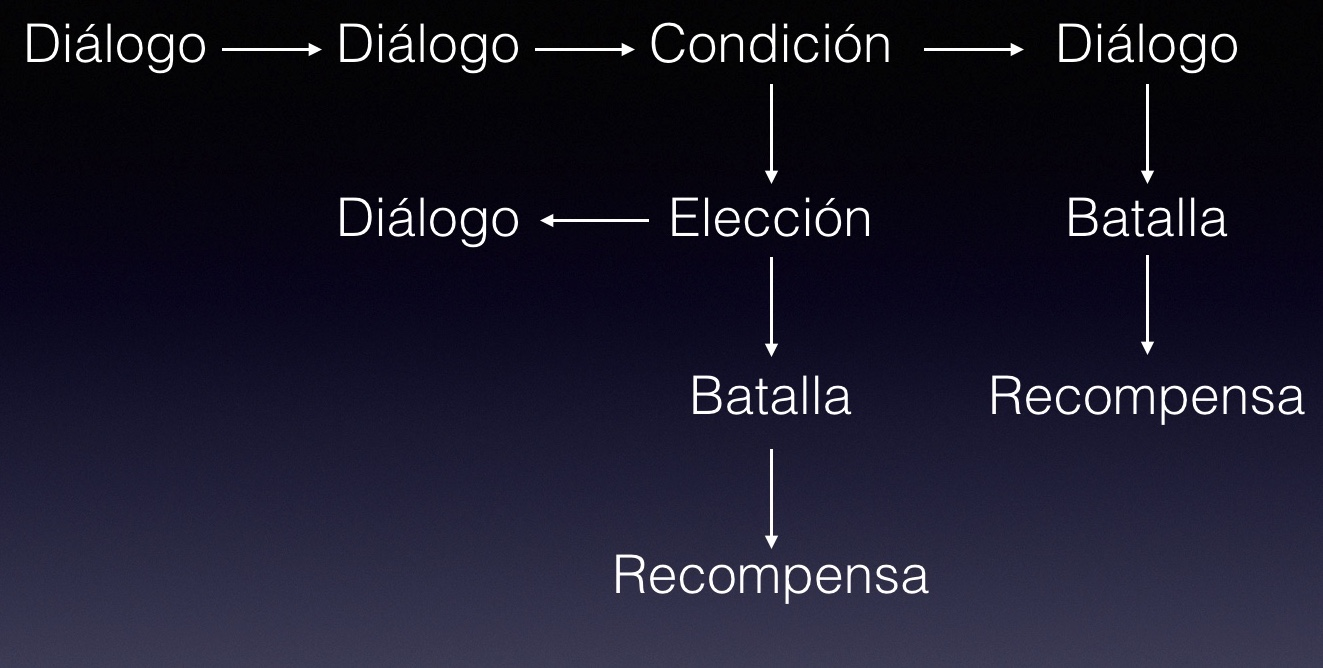
\includegraphics[width=0.75\textwidth]{include/eventsChainExample.jpg}
	
	La idea detrás de los eventos es muy sencilla: al interactuar el usuario con una parte de la aplicación activa una cadena. El evento principal tiene una referencia a otro evento, al que le da paso cuando termina el original. Este encadenamiento sigue hasta que uno de los eventos no tenga ninguna referencia a un evento siguiente, permitiendo que la cadena termine.
\end{figure}

Ahora vamos a definir los tipos de eventos que existen, las acciones que conllevan dentro del motor y sus posibles usos. Respecto a diseño que toman, se describirá más adelante en la sección de diseño \ref{designSection}. 

\subsubsection{Diálogo}
Evento que muestra un mensaje dicho por un personaje en el videojuego. La mayor traba del proyecto original era que los diálogos correspondían con la mayor parte del código fuente, por lo que este evento permite quitar mucha lógica duplicada en el código.

Su uso más frecuente es para mostrar conversaciones entre personajes, aunque también se puede usar para escribir los pensamientos del protagonista, describir una sala o un personaje, plantear un problema...

\subsubsection{Condición}
Evento que verifica una condición sobre el estado actual del juego. Este evento es transparente para el usuario, ya que se ejecutará un evento u otro siguiente dependiendo de si la condición es cierta o no. Las condiciones son las que se describen en la sección \ref{conditionsSubsection}.

Este evento se suele usar cuando se quiere evaluar el estado del juego y tomar acciones en consecuencia. Por ejemplo, diálogos dependientes del compañero, cofres que no se abren si no dispones de una llave...

\subsubsection{Elección}
Evento que permite al jugador escoger entre una serie de opciones. Dependiendo de la opción escogida, se ejecutará un evento u otro. Además, las opciones pueden incluir una condición para que se muestren, como las descritas en la sección \ref{conditionsSubsection}.

Algunos ejemplos en los que aparece este evento son cuando hay que resolver un acertijo y se muestran varias respuestas, o cuando un personaje te ofrece posibles formas de pago para un trueque.

\subsubsection{Batalla}
Evento que inicia una nueva batalla con la información de un enemigo al que enfrentarse.
Hasta que no termine la batalla no se pasará al siguiente evento de la cadena.

Al terminar la batalla se ejecutará un evento según si el jugador ha ganado o ha perdido.

\subsubsection{Recompensa}
Evento que agrega objetos al inventario del jugador.
Se suele usar para recompensar a un jugador por haber ganado una batalla o por haber abierto un cofre.

\subsection{Habitaciones}
La idea original para el desarrollo del juego es un laberinto. Un laberinto se puede representar como una serie de pasillos delgados y oscuros por los que el protagonista debe orientarse, o como una serie de habitaciones interconectadas entre sí.
Esta última opción permite al jugador orientarse por cada partida, obtener mayor detalle sobre los eventos, recordar lugares memorables y ayudar a estructurar el laberinto para el usuario. 

Una habitación es el sitio donde ocurren todos los eventos que se pueden encontrar en el juego. Es en estos lugares donde el jugador va a tener mayor libertad de movimientos porque es el lugar donde se ejecutan cadenas de eventos, puede ir hacia otras habitaciones o donde puede guardar la partida y cambiar ciertos ajustes.

Está representada con una imagen principal que describe a la habitación junto con un título y una descripción, y una serie de acciones que puede realizar el jugador dentro de ella.

\subsection{Personajes}
Durante la aventura el protagonista puede interactuar con múltiples personajes: compañeros, enemigos y NPCs, las siglas de \textit{''non playable character''}. \cite{npcGeekno} Además, el jugador también cuenta como un personaje aparte.

Todos los personajes cuentan con un nombre y una imagen que los representa, y los compañeros y enemigos añaden una serie de características.
Las posibles estadísticas que puede tener un personaje son:

\begin{itemize}
	\item \textbf{Puntos de vida actuales}: representan la vida restante del personaje. Si los puntos de vida actuales del protagonista llegan a 0, entonces el juego termina.
	\item \textbf{Puntos de vida totales}: representan la vida máxima que tiene un personaje.
	\item \textbf{Puntos de ataque}: representan los puntos de vida actuales que puede quitar un personaje con un ataque.
	\item \textbf{Puntos de defensa}: representan los puntos de vida actuales que el personaje elimina de un ataque al recibirlo.
	\item \textbf{Puntos de agilidad}: representan la velocidad de un personaje. En un combate, si un personaje supera por un factor multiplicativo la agilidad del contrario, entonces el personaje puede atacar múltiples veces en un mismo turno. 
	\item \textbf{Estado alterado}: representa un cambio en el estado normal del personaje y pueden reportar beneficios o perjuicios al mismo. Los estados soportados por el motor son veneno, ceguera y parálisis.
	\item \textbf{Arma}: un personaje puede tener un arma consigo para atacar. Estas armas aumentarán el estado base de ataque, añadirán un porcentaje de acierto del ataque y un estado alterado a provocar.
\end{itemize}

Respecto a las tres últimas estadísticas, se explican con más detalle en el apartado de batalla de la sección de diseño \ref{battleDesignSubsection}.

Los personajes por lo tanto son piezas esenciales de la acción durante el juego por distintas razones:

\begin{itemize}
	\item Los diálogos siempre son enunciados por alguien, que debe ser un personaje. Un diálogo no se puede ejecutar si no existe un personaje que lo enuncie.
	\item El protagonista y su compañero tienen una serie de características que son cruciales para la evaluación de condiciones, como los indicadores de habitaciones visitadas.
	\item En una batalla, siempre lucha un personaje enemigo contra el protagonista y sus compañeros.
\end{itemize}

Además, usar personajes permite que los jugadores puedan adentrarse en la aventura con mayor facilidad e incluso identificarse con ellos.

\subsection{Condiciones} \label{conditionsSubsection}
El motor tiene varios puntos donde se necesita ejecutar condiciones para resolver ciertas acciones. Estas condiciones están sujetas a varios factores como las estadísticas del protagonista, valor de las variables internas, etc.

Existen varios tipos de evaluaciones:
\begin{itemize}
	\item Compañero: si el protagonista tiene un compañero que coincide con el nombre definido, entonces la condición se evalúa a verdadera. En otro caso, la condición es falsa.
	\item Objeto: si el protagonista tiene un objeto en su inventario que coincide con el objeto del evento, entonces la condición es cierta. En otro caso, no se cumple la condición. Es importante puntualizar que si la condición es cierta, entonces el objeto del inventario desaparece o se consume.
	\item Estado de habitación: dependiendo si el protagonista ha visitado una habitación específica o no, la condición se evalúa a cierto o falso. Hay una condición que sirve para saber si se ha visitado una habitación y otra para si no la ha visitado.
	\item Relación de variables: si la relación entre dos variables se cumple, entonces la condición es cierta. En otro caso, la condición es falsa. La relación de variables se describe mejor en la sección \ref{variablesSection}.
\end{itemize}

\subsection{Variables personalizadas} \label{variablesSection}
Esta es una nueva funcionalidad del motor que no se encontraba en la original.

Las variables personalizadas es una capacidad del juego que permite almacenar información dinámica de la partida, sin estar limitados por la propia capacidad de evaluar condiciones del motor. Estas permiten a un diseñador de juegos controlar ciertos aspectos internos del desarrollo del juego como puede ser la activación de un evento o de ciertas elecciones.

Estas variables se pueden usar para guardar la información del estado de ejecución de un evento, almacenar la cantidad de tesoros que ha encontrado el jugador durante su partida...

De esta manera, la capacidad de formular condiciones aumenta drásticamente, ya que no dependen de las que puedan estar definidas en el motor. Es más, el diseñador del juego puede emular cualquier condición de las ya definidas si usa las variables correctamente.

Las variables tienen un id que las identifica, el dato que guarda y el tipo de ese dato. Una variable siempre se crea definiendo estos tres campos.
El motor soporta de momento los tipos entero, que representa números enteros; booleano, que representa valores de verdad como verdadero y falso; y cadena de texto, que son un literal de texto.

Debido a que estas variables son dinámicas, el motor permite no solo sustituir el valor o crear nuevas variables, sino que también permite operaciones entre variables u otros datos estáticos.

Las operaciones estarán formadas por dos variables y la operación que realizan entre ellos. El resultado de la operación siempre se guarda en la primera variable con la que se opera. Las operaciones soportadas por el motor dependen del tipo de dato que guarde la variable, y nunca podrán operarse dos variables con distintos tipos de datos.

\begin{itemize}
	\item Las variables \textbf{enteras} soportan las operaciones sustituir, suma, resta, multiplicación, división entera y módulo/resto.
	\item Las variables \textbf{booleanas} soportan las operaciones sustituir, conjunción, disyunción y negación.
	\item Las variables que son \textbf{cadenas de texto} permiten sustituir el texto o concatenarlo.
\end{itemize}

A continuación se describe lo que realiza cada operación:

\begin{itemize}
	\item \textbf{Sustituir}: modifica el valor anterior de la variable con uno nuevo.
	\item \textbf{Disyunción}: ejecuta la operación disyunción booleana sobre la primera y la segunda variable.
	\item \textbf{Conjunción}: ejecuta la operación conjunción booleana sobre la primera y la segunda variable.
	\item \textbf{Negación}: ejecuta la operación negación booleana sobre la segunda variable.
	\item \textbf{Suma}: suma el valor de la primera variable con el de la segunda.
	\item \textbf{Resta}: resta el valor de la primera variable con el de la segunda.
	\item \textbf{Multiplicación}: multiplica el valor de la primera variable por el de la segunda.
	\item \textbf{División entera}: realiza la división entera del valor de la primera variable con el de la segunda.
	\item \textbf{Resto}: halla el resto de la división entera entre el valor de la primera variable y el de la segunda.
	\item \textbf{Sustituir}: concatena el texto de la primera variable con el de la segunda.
\end{itemize}

El uso principal de las variables, cuando ya tienen un valor, es el evaluar su valor comparándolo con otra variable o un dato estático. Para ello, el motor permite realizar operaciones de comparación, y al igual que las operaciones de modificación solo funcionan si los dos tipos de las variables a comparar son iguales. En este caso los operadores son compatibles para todos los tipos de variables, aunque su funcionalidad sea distinta depediendo del tipo.

Los operadores disponibles son igual, distinto, mayor, mayor o igual, menor y menor o igual. A continuación se describe la comparación que se realiza dependiendo del operador.

La condición es cierta:
\begin{itemize}
	\item Operadores enteros:
	\begin{itemize}
		\item \textbf{Igual}: si los dos enteros son iguales.
		\item \textbf{Distinto}: si los dos enteros son distintos.
		\item \textbf{Mayor}: si el primer entero es mayor que el segundo.
		\item \textbf{Mayor o igual}: si el primer entero es mayor que el segundo o si son iguales.
		\item \textbf{Menor}: si el primer entero es menor que el segundo.
		\item \textbf{Menor o igual}: si el primer entero es menor que el segundo o si son iguales.
	\end{itemize}
	\item Operadores booleanos:
	\begin{itemize}
		\item \textbf{Igual}: si los dos valores son iguales.
		\item \textbf{Distinto}: si los dos valores son distintos.
		\item \textbf{Mayor}: si el primer valor es verdadero y el segundo es falso.
		\item \textbf{Mayor o igual}: si el primero es verdadero o si los dos son falsos.
		\item \textbf{Menor}: si el primero es falso y el segundo es verdadero.
		\item \textbf{Menor o igual}: si el primero es falso o si los dos son verdaderos.
	\end{itemize}
	\item Operadores de cadenas de texto:
	\begin{itemize}
		\item \textbf{Igual}: si las dos cadenas son iguales.
		\item \textbf{Distinto}: si las dos cadenas son distintas.
		\item \textbf{Mayor}: si la primera cadena se sitúa posteriormente a la otra según el orden lexicográfico.
		\item \textbf{Mayor o igual}: si la primera cadena se sitúa posteriormente a la otra según el orden lexicográfico o si las cadenas son iguales.
		\item \textbf{Menor}: si la primera cadena se sitúa anteriormente a la otra según el orden lexicográfico.
		\item \textbf{Menor o igual}: si la primera cadena se sitúa anteriormente a la otra según el orden lexicográfico o si las cadenas son iguales.
	\end{itemize}
\end{itemize}

\subsection{Localización}
Supongamos que un diseñador de juegos quiera hacer llegar su juego a la mayor cantidad de gente posible. Aparte de la barrera de los dispositivos que pueden reproducir ese juego, está la barrera del idioma. Aunque ciertos idiomas sean hablados por gran cantidad de gente alrededor del mundo, qué mejor que procurar un juego en el idioma nativo del jugador.

Para ayudar a los diseñadores con este paso, el motor cuenta con soporte para todos los idiomas recogidos en el estándar ISO 639-1 \cite{iso639-1Codes}. Este sistema se ha elegido porque es el estándar que recoge todos los idiomas de forma genérica, sin tener en cuenta diferencias regionales. 

Para ello existen unos ficheros extra donde se pueden definir ciertas claves para ciertos literales de texto que quieren ser traducidos. De esta manera un diseñador puede añadir idiomas extra incluso una vez ya desarrollado el juego. La forma de implementación se describirá en la sección \ref{developmentGuide}.

De ahora en adelante, si se habla de que una funcionalidad es localizable, significa que puede usar una clave que permita traducir el contenido a un idioma.

\newpage
 
\section{Qué esperar del sistema (Diseño)} \label{designSection}
En un mundo en el que todo el mundo puede acceder a miles de aplicaciones a través de un dispositivo portátil que siempre llevan encima y en el que recibir información es lo primordial, es muy importante el diseño que se tiene que llevar a cabo en una aplicación.

Por ello, al desarrollar una aplicación para un teléfono móvil, uno de los factores clave es que sea muy atractiva, bonita y usable.
En esta sección se describirán las elecciones de diseño que se han llevado a cabo para las funcionalidades visuales del motor, dividiéndolas en pantallas visuales. Están adjuntas capturas de la propia aplicación para ayudar a la comprensión de ciertas decisiones.

\subsection{Pantalla de menú principal}
\begin{center}
	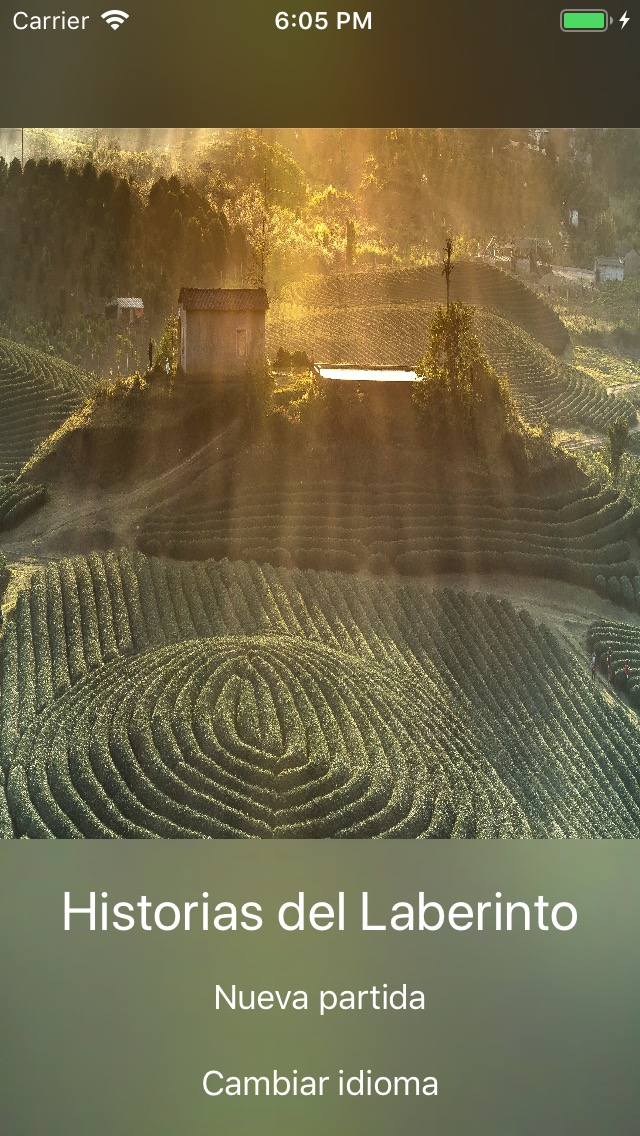
\includegraphics[width=0.3\textwidth]{include/snapshots/mainMenu-es.jpg}
	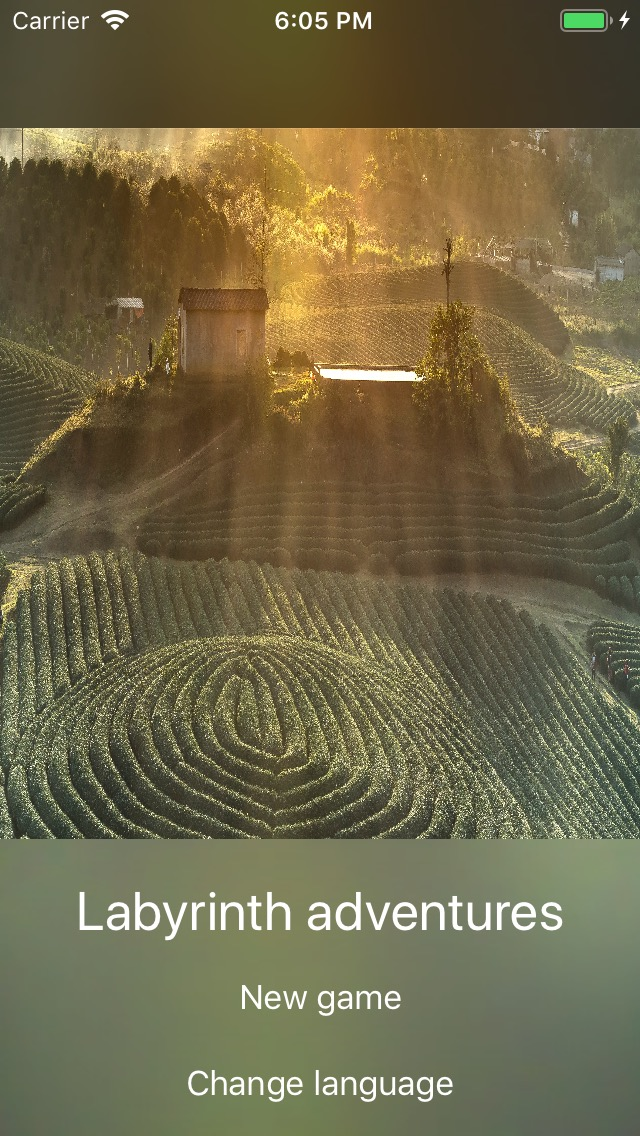
\includegraphics[width=0.3\textwidth]{include/snapshots/mainMenu-en.jpg}
\end{center}
El menú principal es la primera pantalla de la aplicación. Sirve para iniciar la partida cargada, continuar una partida o cambiar el idioma del juego. Debido a que es la primera pantalla del motor, está incluida una imagen con grandes cultivos que asemejan a un laberinto. Esta imagen no se puede cambiar, está fija y no depende del juego cargado.

Nada más cargarse la aplicación, se cargan los ficheros de texto del juego cargado y se escoge un idioma.
El idioma que se elige depende del usuario: si es la primera vez que carga la aplicación, se escogerá uno que corresponda con algún idioma configurado en el dispositivo. En otro caso, usa el lenguaje usado por última vez en la aplicación.

A continuación se describe la acción que debe realizar cada botón:

\begin{itemize}
	\item \textbf{''Nueva partida''}: permite iniciar una nueva partida. Para ello, el motor mostrará una pantalla de carga mientras se encarga de descodificar los ficheros iniciales del juego, guardar la información en la base de datos, inicializar ciertos parámetros y cargar en disco las imágenes que se puedan descargar de Internet.
	\item \textbf{''Cargar partida''}: recupera el estado de una partida guardada anteriormente. Como todos los datos ya están cargados en la base de datos, directamente aparece el lugar en el que estuviera el jugador anteriormente.
	\item \textbf{''Cambiar idioma''}: permite cambiar el idioma de la aplicación. Al pulsar navega directamente a la pantalla de cambio de idioma.
\end{itemize}

\subsection{Pantalla de cambio de idioma}
\begin{center}
	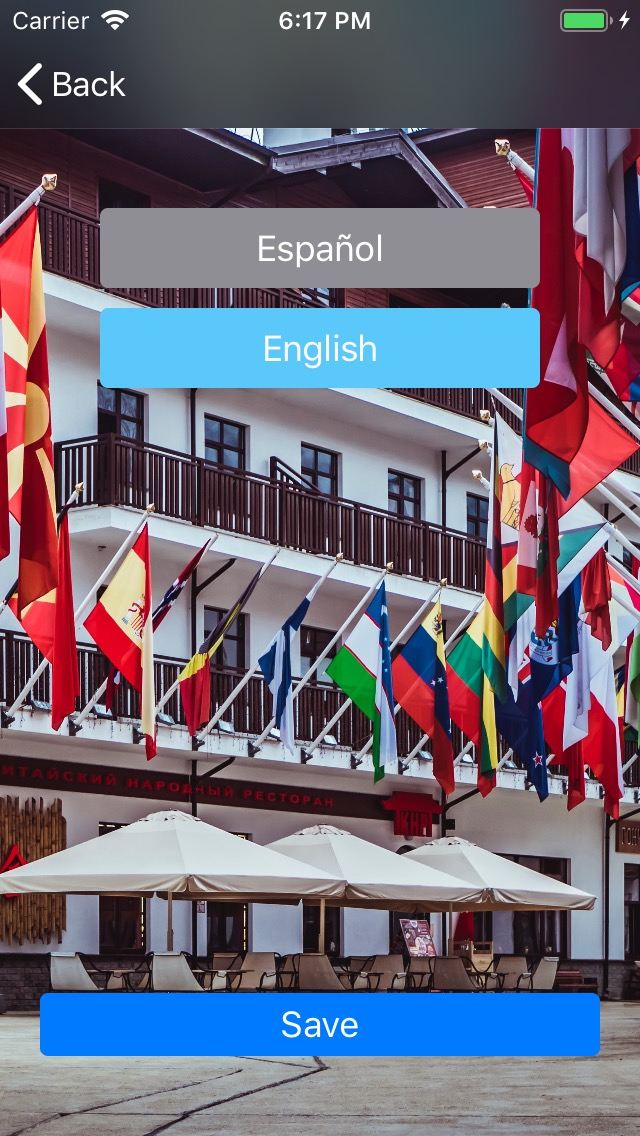
\includegraphics[width=0.3\textwidth]{include/snapshots/languageSettings.jpg}
\end{center}
En esta pantalla se permite al usuario cambiar el idioma entre una lista de idiomas soportados en ese momento por el motor. La aplicación soporta cualquier lenguaje recogido en el estándar ISO 639-1 \cite{iso639-1Codes}.

El fondo no se puede cambiar, aunque muy posiblemente cambie en un futuro muy cercano.
El idioma seleccionado actualmente es el que está marcado en azul. Un jugador puede seleccionar cualquier otro idioma para cambiar la selección, aunque los cambios no se guardan hasta que el usuario pulse el botón de guardado en la parte inferior.
Al pulsar guardar, se recarga la aplicación para que muestre todos los textos en el idioma seleccionado. 

\subsection{Pantalla de habitación}
\begin{center}
	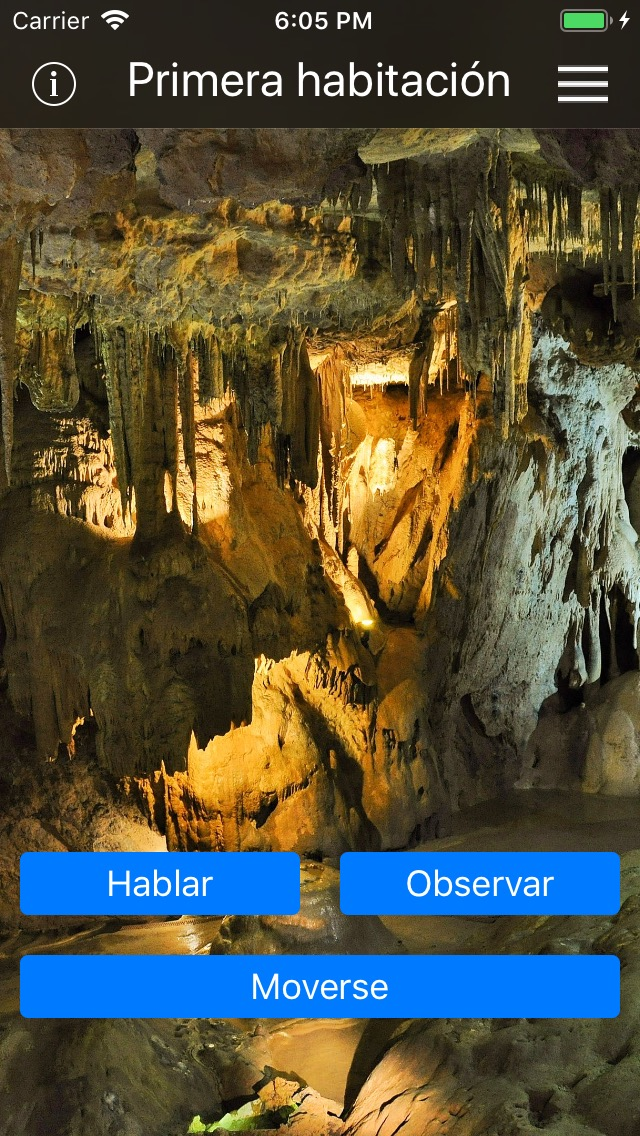
\includegraphics[width=0.3\textwidth]{include/snapshots/roomView.jpg}
	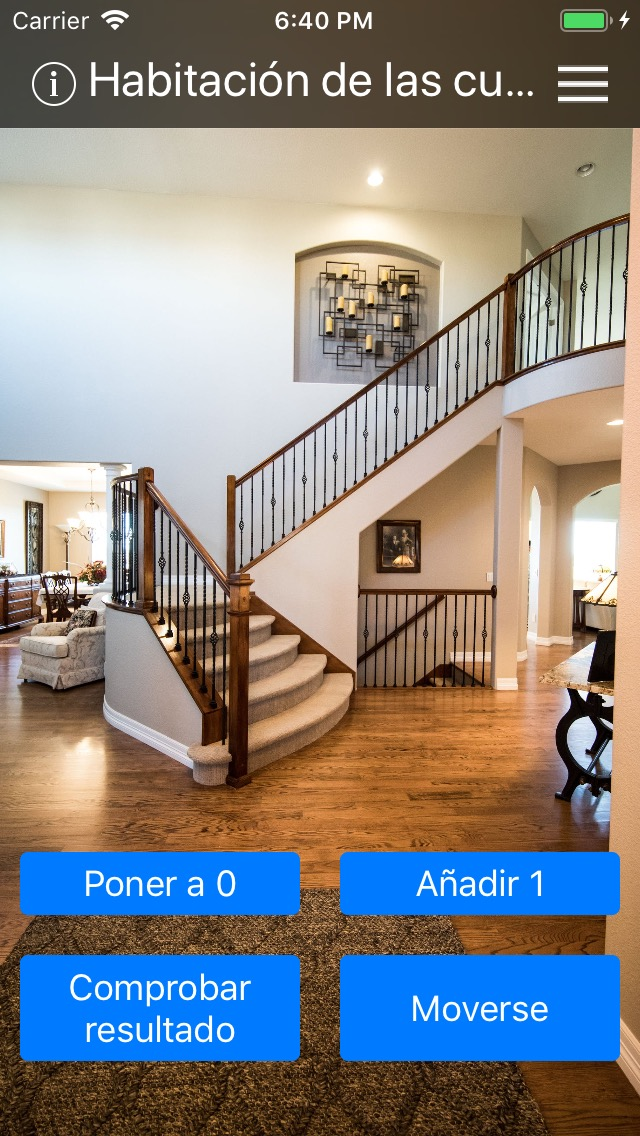
\includegraphics[width=0.3\textwidth]{include/snapshots/secondRoomView.jpg}
\end{center}

La pantalla de habitación es donde se desarrolla la mayor parte de los eventos del juego y es donde el jugador pasará más tiempo en una partida.
Esta pantalla es la encargada de gestionar las acciones principales del jugador: moverse entre otras habitaciones, abrir el menú secundario y ejecutar eventos según una serie de acciones incluidas en la habitación.

La vista cuenta con botones de acción en la parte inferior, un botón de información y un botón de bocadillo. Además el nombre de la misma está escrita en la parte superior, y la imagen de fondo cambia según la habitación en la que se encuentre el usuario.

Esto es lo que ocurre si se pulsan en los distintos botones:
\begin{itemize}
	\item \textbf{Botón de información}: situado en la esquina superior izquierda, el botón de información muestra un diálogo que describe a la habitación en la que se encuentra el jugador.
	\item \textbf{Botón de bocadillo}: situado en la esquina superior derecha, lleva al jugador al menú secundario.
	\item \textbf{Eventos}: las acciones de eventos son los botones azules que siempre están en la parte inferior de la pantalla y representan las acciones que puede realizar el jugador en esa habitación. Al pulsar en uno de ellos, se ejecuta el evento que contenga.
	\item \textbf{''Moverse''}: es el botón azul que está ubicado en la parte inferior de la pantalla como la última acción. Pulsarlo lleva al usuario a la pantalla de movimiento o de cambio de sala.
\end{itemize}

Normalmente una habitación cuenta como máximo con cuatro acciones, incluyendo la de ''Moverse'', aunque soporta muchas acciones, técnicamente infinitas. Cuando aparezcan más de cuatro acciones, entonces la vista de los botones se podrá desplazar para mostrarlos todos.

\subsection{Pantalla de movimiento}
\begin{center}
	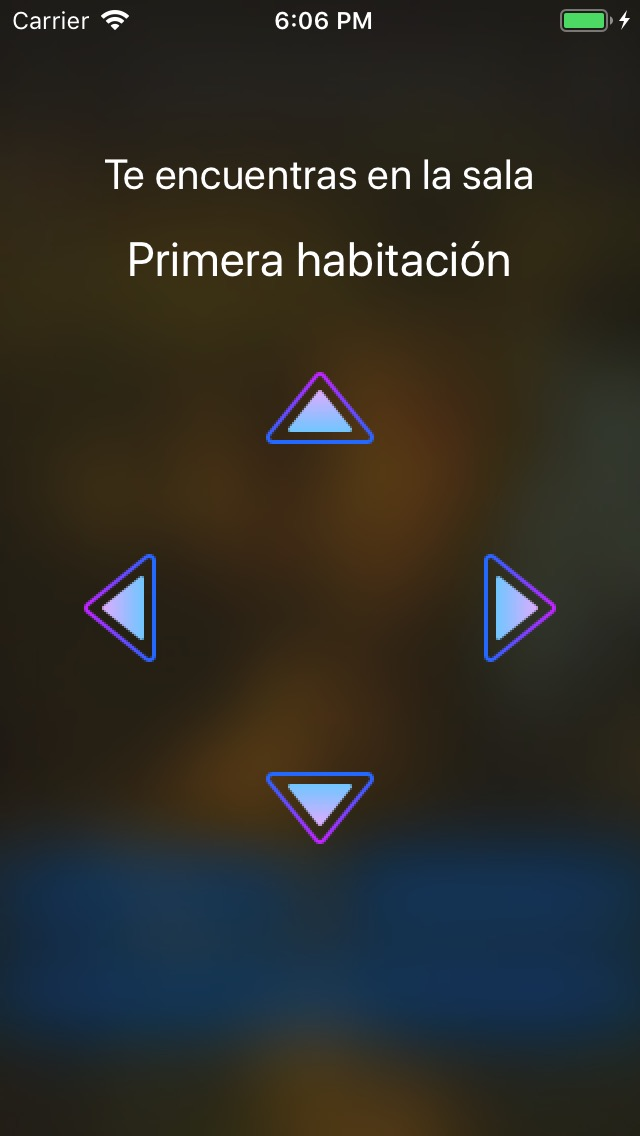
\includegraphics[width=0.3\textwidth]{include/snapshots/movementView.jpg}
	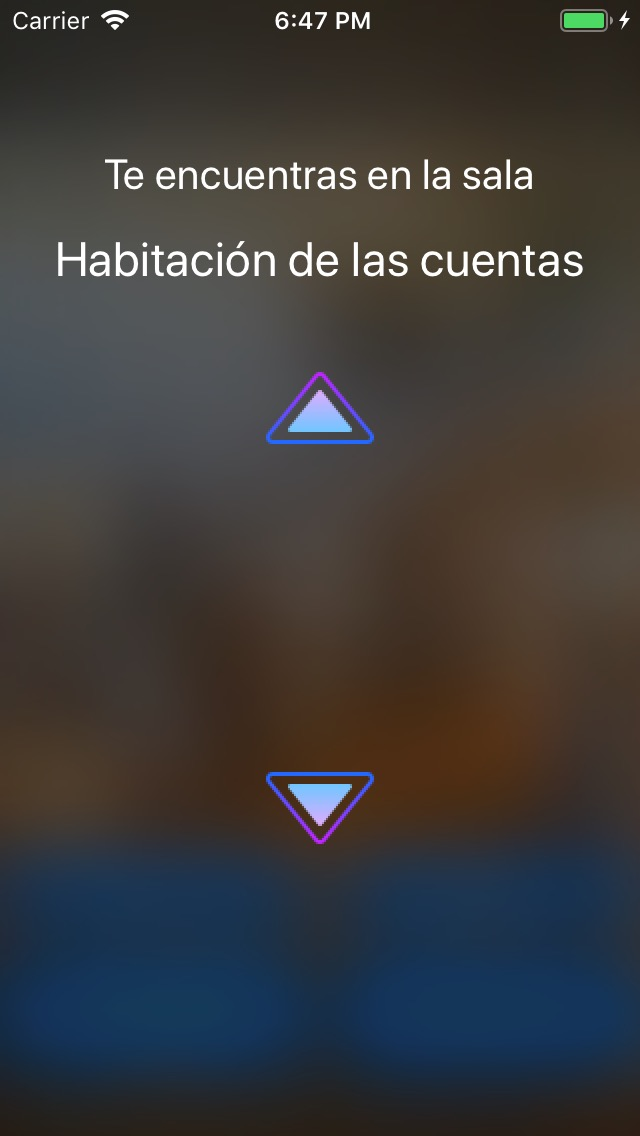
\includegraphics[width=0.3\textwidth]{include/snapshots/movementView_2.jpg}
\end{center}

La pantalla de movimiento permite al jugador cambiar la posición de su personaje y navegar en el laberinto de habitaciones.
Se muestra una pantalla que se superpone a la de la habitación y que contiene el nombre de la habitación en la que se encuentra el usuario y unas flechas que le permiten elegir hacia qué dirección quiere moverse.

Al pulsar en una de las flechas, el jugador se moverá a la habitación que se encuentre en esa dirección, por lo que saldrá de la vista de movimiento y cambiará a la nueva habitación.

El mapa del laberinto es aleatorio, cada vez que el usuario elija una habitación en la que todavía no ha estado presente, el motor recogerá una habitación que no se haya visitado de entre todas las habitaciones configuradas en el juego y fijará su posición, por lo que el jugador podrá volver a visitarla si vuelve al mismo lugar.
Mientras el laberinto tenga varias salas disponibles sin visitar, el movimiento estará disponible en cualquier dirección.
 
En ciertas ocasiones el motor usará una habitación genérica en lugar de las habitaciones configuradas con el propósito de alargar el juego con eventos genéricos determinados por el diseñador. Estas salas normalmente tienen eventos como un cofre con contenido común, un enemigo débil...

Hay que resaltar que en el juego original el jugador cambiaba la dirección a la que miraba cada vez que se movía, simulando un movimiento real de forma más fiel, y para orientarse contaba con una brújula que le permitía saber hacia que punto cardinal estaba mirando.
Sin embargo, en esta aplicación todavía no se ha implementado esta funcionalidad, por lo que no existe este sistema de giro, el jugador siempre estará mirando hacia el mismo sitio.

\subsection{Menú secundario}

\subsection{Inventario}

\subsection{Ejecución de eventos}
La aplicación realiza una acción dependiendo del tipo de evento que se vaya a ejecutar. Algunas de estas acciones muestran una vista que las representa y otras se mantienen invisibles, transparentes para un jugador.

A continuación se describe la acción que realiza cada uno de los eventos, dependiendo del tipo:

\subsubsection{Diálogo}
\begin{center}
	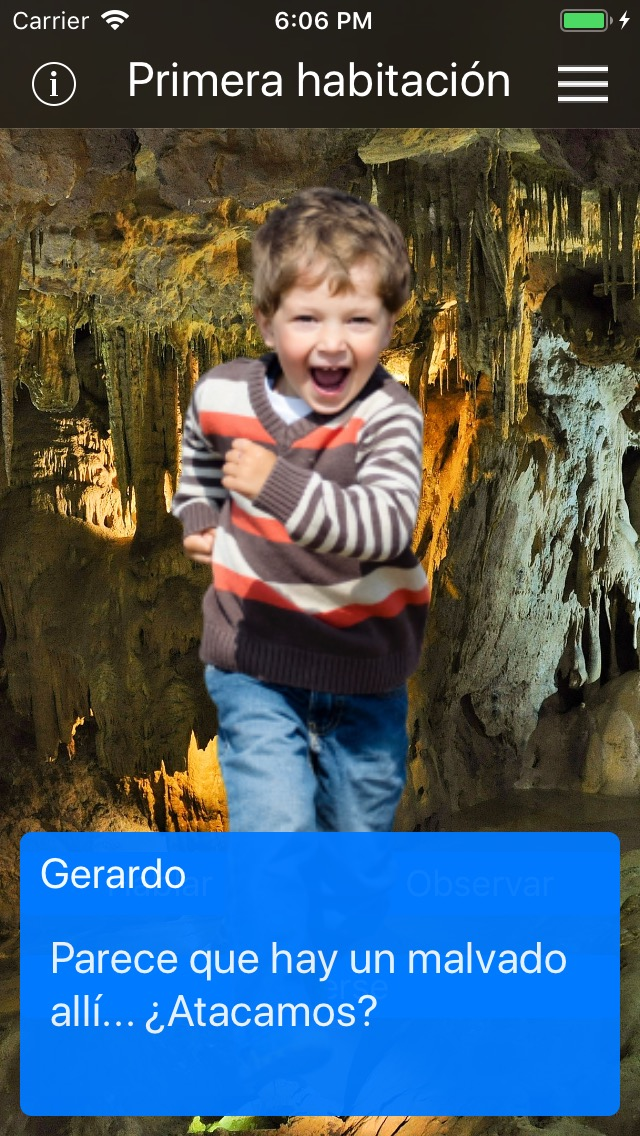
\includegraphics[width=0.3\textwidth]{include/snapshots/dialogue.jpg}
\end{center}
Este evento está encargado de mostrar un mensaje para que el jugador pueda leerlo. Para ello, la aplicación muestra una pantalla por encima de la sala actual, el jugador se mantiene en la misma sala, con ciertas características:

\begin{itemize}
	\item Mensaje: se muestra el mensaje recogido en el evento. Este mensaje es localizable, por lo que se puede traducir a cualquier idioma.
	\item Personaje: se muestra el nombre y la imagen de un personaje, para que el jugador reconozca quién está diciendo el mensaje.
\end{itemize}

Aunque la interfaz de la sala siga viéndose por detrás del diálogo, no se puede interactuar con ella.
Si el usuario pulsa en cualquier sitio de la pantalla, se ejecutará el siguiente evento.

\subsubsection{Condición}
Una condición es un evento transparente para el usuario, no se realizará ningún cambio en la UI. Sin embargo, como realiza operaciones rápidas no bloquea la experiencia de usuario.

\subsubsection{Elección}
\begin{center}
	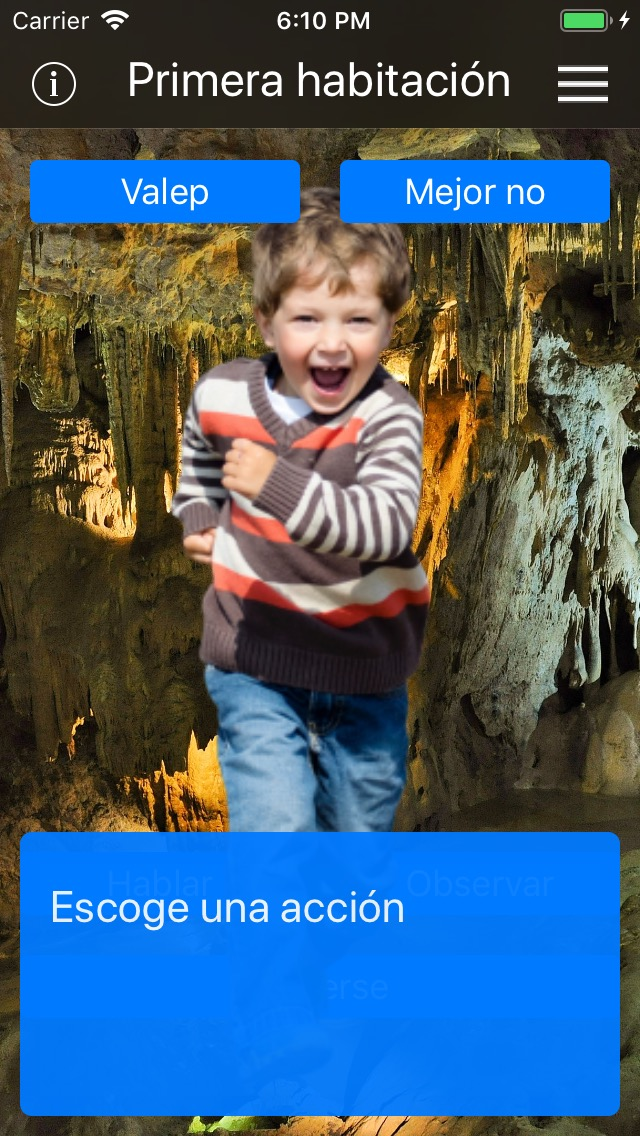
\includegraphics[width=0.3\textwidth]{include/snapshots/chose.jpg}
\end{center}
La elección permite a un usuario recuperar el control de la aplicación y escoger entre una serie de acciones descritas por el evento. Estas opciones aparecen si la condición que tienen anexa se cumple o si no tienen condición.

Muestra un mensaje localizable que insta al jugador a escoger una opción de entre las seleccionadas. Además aparece la imagen del personaje usado en un evento anterior.

El jugador solo puede pulsar en uno de los botones que aparecen con las posibles elecciones. Si el usuario pulsa en cualquier otro sitio, no ocurrirá nada.
Al pulsar en una de estas opciones, se ejecutará el evento que corresponda.

\subsubsection{Batalla} \label{battleDesignSubsection}
\begin{center}
	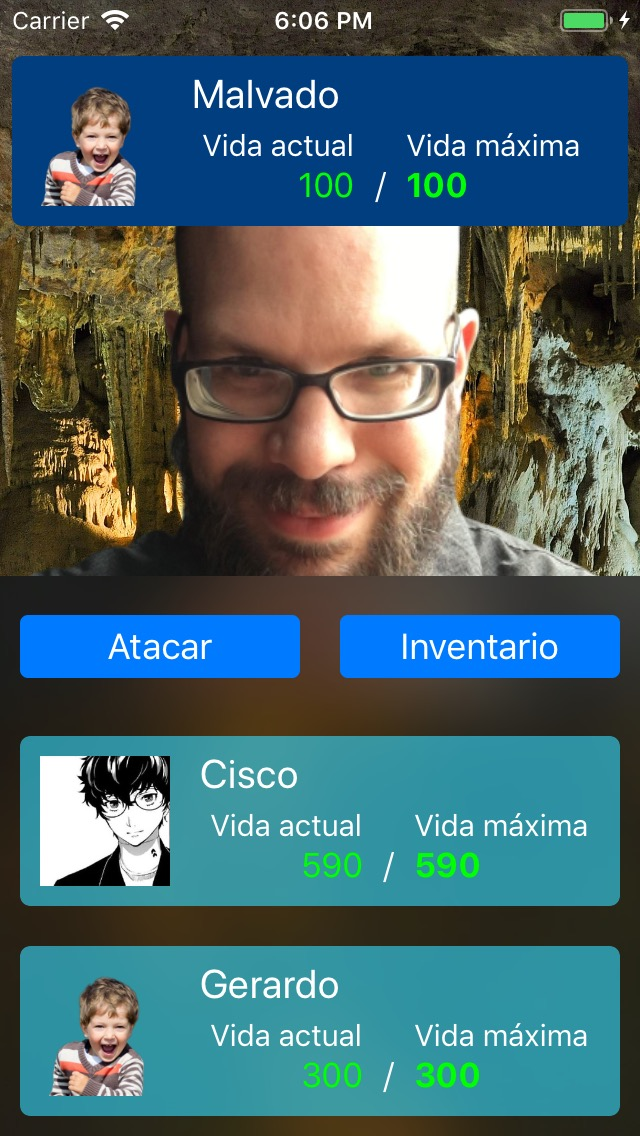
\includegraphics[width=0.3\textwidth]{include/snapshots/battle.jpg}
\end{center}
La batalla es una parte muy importante de la aplicación, ya que es uno de los lugares donde un jugador va a poder salir de la dinámica de explorar la mazmorra y entrar en otra dinámica del juego.
Además, debido a que el planteamiento del combate es muy simple, se necesita que la interfaz sea lo más atractiva posible y que el combate en sí sea suficientemente fluido.

Un combate muestra a dos equipos enfrentados, el equipo del jugador contra el del enemigo. El equipo del jugador tiene que atacar al enemigo y viceversa, reduciendo sus puntos de vida actuales respectivamente. Un luchador se considera derrotado cuando sus puntos de vida actual llegan a 0.

Gana el primer equipo que acabe con el representante del otro equipo, es decir, gana el equipo del enemigo si acaba con el protagonista y gana el equipo del protagonista si acaba con el enemigo principal.

En el combate solo participan personajes jugables, es decir, personajes que contengan estadísticas. Si se intenta comenzar una batalla con un personaje que no tenga estadísticas, el evento de batalla no funcionará.

Respecto a la pantalla, debido a que en un combate se representa la lucha entre dos equipos, hay una mitad de pantalla para cada equipo.
En la parte superior se encuentra el bando enemigo. Se muestra una vista de estado con la información del enemigo y una imagen que representa al enemigo principal.
En la parte inferior se encuentra el bando del jugador, mostrando las ventanas con la información de sus luchadores y dos botones que permiten al jugador realizar acciones.

También se puede observar 3 cuadrados de información, dos para el equipo de jugador y uno para el enemigo. En este caso, los dos equipos muestran esencialmente lo mismo. Aquí se describe qué indica cada dato de esta vista:
\begin{itemize}
	\item Nombre y foto del personaje: permite reconocer a cada luchador en la batalla. Cada luchador debería tener su propio nombre y foto para evitar confundir al jugador.
	\item Vida actual: representa la vida actual de la que dispone en el momento el luchador. Esta se reduce si un luchador contrario ataca al luchador, por lo tanto el número varía.
	Además, los puntos de vida siguen un código de colores para ayudar al jugador a darse cuenta del estado en el que se encuentra ese luchador: si el color es \textcolor{green}{verde} significa que los puntos de vida actuales están al máximo, si el color es \textcolor{yellow}{amarillo} significa que los puntos están por debajo de un cuarto del máximo, si el color es  \textcolor{red}{rojo} significa que tiene 0 puntos, y en otro caso el color será blanco.
	\item Vida máxima: representa el tope de vida que tiene un luchador.
	\item Estado alterado: situado en la esquina superior derecha, representa el estado alterado que puede sufrir uno de los personajes. Si el personaje no tiene ningún estado alterado, entonces no aparece información al respecto.
\end{itemize}

Durante una batalla, el jugador solamente podrá controlar a su personaje, al protagonista. El resto de acciones, las realizadas por el resto del equipo del jugador y el equipo del enemigo, son calculadas automáticamente por la aplicación. 

Respecto a las dos botones, representan las dos acciones que puede realizar un usuario.
\begin{itemize}
	\item Atacar: realiza la acción de atacar sobre el enemigo.
	\item Inventario: lleva al usuario a la vista de inventario, para permitirle usar objetos de la misma manera que desde el menú secundario.
\end{itemize}

La batalla está diseñada prácticamente igual a la que se encontraba en el juego original. Aunque esta vez la aplicación cuente con una interfaz que representa mejor una pelea, el núcleo lógico de toda la pantalla es muy parecido al anterior. De todas maneras, a continuación se describe cómo está diseñada la vista, funcionalmente hablando. 

El combate sigue siendo por turnos, siguiendo el orden original: primero actúa el protagonista, después el enemigo y por último el resto del equipo del jugador. Cada turno cuenta con una serie de fases que le permite al jugador darse cuenta de lo que está ocurriendo. En esta descripción, siempre se hablará del personaje que actúa en el turno como luchador y contrario como el personaje al que ataca el responsable del turno.

\begin{enumerate}
	\item Fase de continuidad de estado alterado: el motor analiza el estado del luchador, y si tiene un estado alterado evalúa que el luchador pueda perder ese estado alterado.
	\item Fase de evaluación de daño de estado alterado: el motor analiza el estado del luchador y realiza ciertas acciones si tiene un estado alterado específico. Si el luchador está envenenado, entonces le hace una cantidad de daño al luchador; y si está paralizado hay una probabilidad de que pierda su turno.
	\item Fase de introducción de acción: el motor pregunta al luchador qué acción quiere realizar. Si el luchador es el protagonista, el jugador podrá elegir una de las acciones descritas anteriormente en los botones. En otro caso, el luchador siempre decidirá atacar al contrario.
	\item Fase de ataque: el motor comienza el cálculo del ataque. Si no se dispone de objetivo, el motor elige uno aleatoriamente del equipo contrario de entre los que están vivos, es decir, tienen más de 0 puntos de vida actuales. Tras ello, el motor calcula el daño que recibe el objetivo a partir de las estadísticas del luchador y el contrario. Se explica con más detalle esta fase más adelante.
	Además, si el luchador cuenta con el estado alterado ceguera, entonces es posible que falle el ataque.
	\item Fase de evaluación de daño contrario: el motor analiza el estado del contrario y evalúa si está derrotado.
\end{enumerate}

Esta cadena de turnos se repite hasta que se da el caso de que uno de los representantes de los equipos sea derrotado. Si el representante del equipo enemigo ha sido derrotado, entonces se activa el evento de victoria. Si el protagonista es el derrotado, entonces se activa el evento de derrota.

Por último, ya que la fase de ataque es más compleja que el resto, se va a describir qué realiza exactamente el motor en esa fase:
\begin{enumerate}
	\item Fase de obtención de arma: el motor evalúa si el luchador tiene un arma con la que luchar. Si es así, la carga en el sistema. Esta arma permite al luchador obtener modificadores de fuerza, estado alterado y acierto, por lo que modifica la fuerza del luchador, permite inflingir estados alterados al objetivo y tiene un porcentaje que determina si el luchador acierta un ataque.
	\item Fase de cálculo de golpes: el motor se basa en la relación entre la agilidad del luchador y de su objetivo para calcular el número de golpes que efectuará el luchador. Para ello realiza la división entera entre la agilidad de los dos, y el resultado es el número de golpes que el luchador puede realizar.
	Después, calcula si el luchador puede fallar alguno de esos golpes. Si este no tiene arma, entonces acierta todos los golpes. En otro caso, usará el porcentaje definido en el arma para calcular los golpes que da.
	\item Fase de cálculo de daño: si el luchador acierta ningún ataque, entonces termina su turno. Si consigue acertar, entonces se calcula el daño teniendo en cuenta la fuerza del luchador y la defensa del enemigo, aparte del factor de fuerza extra que puede reportar un arma.
	\item Fase de cálculo de estado alterado: si el luchador ha conseguido conectar algún golpe y además lleva un arma equipada que puede causar un estado alterado, entonces hay una probabilidad de que se lo cause al objetivo.
\end{enumerate}

\subsubsection{Recompensa}
\begin{center}
	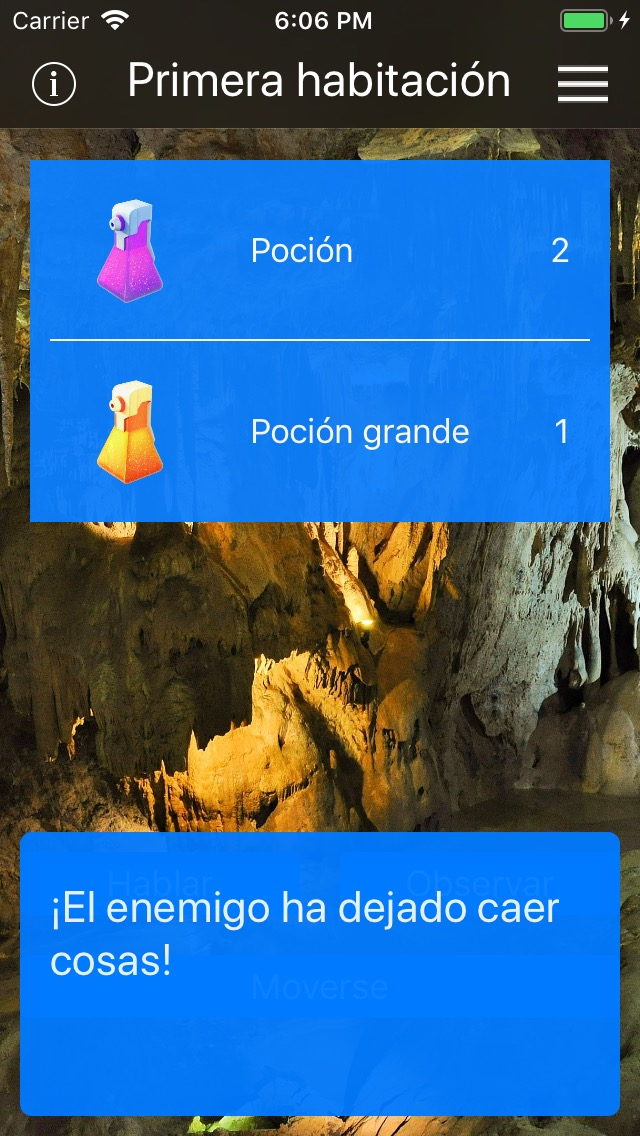
\includegraphics[width=0.3\textwidth]{include/snapshots/reward.jpg}
\end{center}
La recompensa muestra al usuario una serie de objetos que consigue, especificados en el evento.
En la parte inferior se muestra un mensaje localizable del evento. En la parte superior se muestra una lista de objetos obtenidos por el jugador. Teóricamente un jugador puede recibir tantos objetos como se especifique en el evento.
Cada objeto está representado con su nombre localizable, una cantidad que se recibe y una foto indicando qué objetos se reciben.

\section{Cómo crear un videojuego} \label{developmentGuide}
En esta sección se define cómo crear un juego que sea compatible con el motor. Para ello, se dispone de una serie de ficheros que permiten a la aplicación cargar la información básica y empezar el juego. En esta sección se explicará para qué sirve cada fichero y cómo se deben rellenar.

Estos ficheros tienen formato YAML \cite{yamlDocumentation}. Este formato permite la manipulación de datos serializables de forma sencilla tanto por el programador como por un usuario, es decir, son ficheros fáciles de transformar a código y son fáciles de interpretar y diseñar por una persona. 
% $\lq hola \lq 
Un fichero de este tipo sigue un formato ''clave:valor''. Todas las claves están definidas en inglés, para permitir que los diseñadores puedan tener un lenguaje común para crear juegos.
Algunas claves son opcionales. Si una clave es opcional, significa que puede no aparecer o aparecer vacía.

\subsection{Imágenes}
Un diseñador puede crear o descargar sus propias imágenes para usarlas en el juego. Para ello existe una carpeta llamada ''images'', donde se deben guardar las imágenes necesarias.
En todo caso, si el diseñador prefiere generar un juego de manera que sus elementos no pesen demasiado, el motor también soporta la descarga de imágenes por Internet, siempre teniendo en cuenta que sólo puede descargar imágenes de URLs con soporte SSL a través del protocolo HTTPS, es decir, que comiencen por ''https''.
El motor acepta archivos con tipos comunes, como JPEG o PNG. No se asegura la compatibilidad con otros tipos de ficheros.

Para representar una imagen hay que especificar el origen de la imagen y el lugar donde se encuentra el recurso. El origen puede ser tanto local como remoto. Si el origen es local, el diseñador debe especificar el nombre del fichero al que quiere acceder. Si el origen es remoto, el diseñador debe especificar la URL que contiene la imagen.

\begin{lstlisting}
#Si el fichero es remoto:
imageSource:
	type: remote
	source: "https://imgur.com/zNGi05P.png"
	
#Si el fichero es local:
imageSource:
	type: local
	source: "tarta.jpg"
\end{lstlisting}

\subsection{Literales localizables}
En la pantalla de cambio de idioma se hacía referencia a la posibilidad de definir literales de texto que podían ser traducidos. Un literal suele ser una frase que resume la traducción del texto. Normalmente se encuentran de la forma "literal" = "traducción".

La información de los idiomas se guarda en la carpeta ''texts'', donde se encuentra un fichero para cada idioma que se quiera implementar. Estos ficheros son los que albergan esos literales y sus traducciones. Es importante repetir que solo se puede usar un fichero para cada idioma, es decir, si se quiere que el juego esté disponible en español e inglés, entonces en la carpeta ''texts'' debe haber dos ficheros, uno para el español y otro para el inglés.

Los archivos deben llamarse siempre <codigo\_iso639-1\_del\_idioma>.strings \cite{iso639-1Codes} para que el sistema sea capaz de reconocerlos.
A continuación se muestra un ejemplo de cómo se deben rellenar:

\begin{lstlisting}
#es.strings
"newGameButton" = "Nueva partida";
"loadGameButton" = "Cargar partida";
"gameTitle" = "Historias del Laberinto";
"changeLanguageButtonText" = "Cambiar idioma";
"room17LookAroundMessage" = "Miras a tu alrededor";

#en.strings
"newGameButton" = "New game";
"loadGameButton" = "Load game";
"gameTitle" = "Labyrinth adventures";
"changeLanguageButtonText" = "Change language";
"room17LookAroundMessage" = "You take a look at your surroundings.";
#Los ; situados al final son muy importantes para que los textos puedan ser cargados.
\end{lstlisting}

Para añadir un texto localizable a cualquier parte del juego, hay que usar el literal en vez de su traducción.
\begin{lstlisting}
#En vez de poner una traduccion directa en el fichero correspondiente...
- id: "room17LookAround"
	mode: "dialogue"
	message: "Miras a tu alrededor"
	characterId: "narrator"
	nextStep: "room17LookAround2"

#se usa el literal.
- id: "room17LookAround"
	mode: "dialogue"
	message: "room17LookAroundMessage"
	characterId: "narrator"
	nextStep: "room17LookAround2"
\end{lstlisting}

\subsection{Condiciones}
No existe un fichero específico para las condiciones, implicaría más complicación para desarrollar los ficheros, aunque permitiría añadir orden.
Sin embargo, se añade esta subsección para hablar de cómo modelizar condiciones en los ficheros. Todas las condiciones se modelan igual en todos los sitios, para evitar confusiones.

\begin{lstlisting}
# Existen varios tipos de condiciones:
# Companero
condition:
	kind: "partner"
	required: "gerar" # Id del companero que sigue al protagonista.
	
# Objeto
condition:
	kind: "item"
	required: "potion" # Id del objeto que tiene que tener el protagonista. Si se cumple esta condicion, entonces el protagonista perdera una unidad de ese objeto.
	
# Habitacion visitada
condition:
	kind: "roomVisited"
	required: "startRoom" # Id de una sala. Es cierta si la sala ya se ha visitado.
	
# Habitacion sin visitar
condition:
	kind: "roomNotVisited"
	required: "startRoom" # Id de una sala. Es cierta si la sala todavia no se ha visitado.
	
# Variables
condition:
	kind: variable
	required:
		compareToId: "numberOfApples" # Id de la variable del lado izquierdo de la comparacion.
		relation: equal # Operacion de relacion entre las variables.
		initialVariable: # Opcional. Variable con informacion estatica para el lado derecho de la comparacion. Si este campo no aparece, debe aparecer el de la siguiente condicion. En otro caso, no funcionara el evento que contenga esta condicion.
			type: integer
			value: 10
		
condition:
	kind: "variable"
	required:
		compareToId: "numberOfApples"
		relation: equal
		initialVariable: "cupcakes" # Opcional. Id de la variable del lado derecho de la comparacion. Si este campo no aparece, debe aparecer el de la condicion anterior. En otro caso, no funcionara el evento que contenga esta condicion.

\end{lstlisting}


\subsection{Personajes}
Este fichero define todos los personajes que van a aparecer a lo largo del juego, junto con toda la información que necesiten. Se debe llamar ''characters.yml''.

\begin{lstlisting}
playable: #Incluye los personajes con estadisticas de combate.
	"gerar": #Id del personaje. Debe ser unico. Representa al personaje
		name: "Gerardo" #Nombre del personaje. Este se mostrara en el juego. Localizable.
		currentHealthPoints: 300 #Puntos de vida actuales. Este dato solo sirve para el principio del juego, no representa el estado del juego.
		maxHealthPoints: 300 #Puntos de vida maximos.
		attack: 15 #Puntos de ataque.
		defense: 15 #Puntos de defensa.
		agility: 4 #Puntos de agilidad.
		weapon: "magic_sword" # Opcional. Indica el id del arma que porta el protagonista.
		imageSource: #Imagen grande del personaje. Se usa en dialogos.
			type: remote
			source: "https://imgur.com/zNGi05P.png"

		portraitSource: #Imagen reducida del personaje. Se usa en la vista de estado del personaje.
			type: remote
			source: "https://i.imgur.com/g3WIUf4.png"

notPlayable: #Incluye los personajes que no tienen estadisticas de combate. Aunque se incluya a un personaje con estadisticas aqui, no se podra usar como personaje en batallas.
	"narrator": #Id del personaje. Debe ser unico. Representa al personaje.
		name: "Narrador" #Nombre del personaje. Este se mostrara en el juego. Localizable.
		imageSource:  #Imagen grande del personaje. De tipo remoto.
			type: remote
			source: "https://i.imgur.com/Upcm999.png"

	"aurelionSol":
		name: "Aurelion Sol"
		imageSource: #Imagen grande del personaje. De tipo local.
			type: local
			source: "aurelionSol.PNG"
\end{lstlisting}

Todas las estadísticas que se rellenen con números deben ser enteros. El motor no funcionará si se incluye un número con decimales.

\subsection{Protagonista}
El protagonista, el personaje controlado por el jugador, tiene su propio fichero. Muchas de las estadísticas son iguales, pero tiene cierta información extra. El nombre del fichero es ''prota.yml''.

\begin{lstlisting}
name: "Cisco" # Nombre del protagonista. Localizable.
partner: "gerar" # Opcional. Id del personaje que viaja con el protagonista. Debe ser un personaje con estadisticas.
imageSource: # Imagen grande del protagonista.
	type: remote
	source: "https://vignette.wikia.nocookie.net/megamitensei/images/6/63/Persona_5_Hero.png"
portraitSource: # Imagen reducida del protagonista.
	type: remote
	source: "https://vignette.wikia.nocookie.net/megamitensei/images/1/14/P5_manga_Akira.jpg"

currentHealthPoints: 590 # Puntos de vida actuales. Este dato solo sirve para el principio del juego, no representa el estado del juego.
maxHealthPoints: 590 # Puntos de vida maximos.
attack: 30 # Puntos de ataque.
defense: 10 # Puntos de defensa.
agility: 10 # Puntos de agilidad.
weapon: "magic_sword" # Opcional. Indica el id del arma que porta el protagonista.
	
items: # Objetos que porta el protagonista al principio de la aventura.
	"potion": 1 # Este objeto tiene el id del objeto como clave y la cantidad de la que se dispone como valor.
	"high_potion": 2
	"small_key": 1
\end{lstlisting}

El protagonista no tiene id, por lo que su id es siempre "prota".

\subsection{Objetos}
El fichero de objetos recoge todos los objetos que se pueden encontrar a lo largo de una partida. Se guardan en un archivo llamado ''items.yml''.

Los objetos tienen un id, un nombre, una descripción, un tipo y una imagen asociada. Hay tres tipos de objetos: consumibles, armas y clave.
\begin{itemize}
	\item Consumibles: incluyen un campo obligatorio que indica la cantidad que aumenta o disminuye los puntos de vida actuales de un personaje.
	\item Objetos clave: representan un objeto que se usará para ciertas condiciones. No tienen más campos.
	\item Armas: objetos que usan los personajes para atacar. Podrán tener opcionalmente una estadística de fuerza extra, un porcentaje de acierto y un estado alterado que provocan junto con un porcentaje de provocarlo. Si no está el campo de fuerza extra, se supondrá que es 0. Si no está el campo de estado alterado, se supondrá que es "ninguno". 
\end{itemize}

Si un objeto aparece en algún sitio y no está en este fichero, entonces se tratará como si no estuviera dentro del inventario.

\begin{lstlisting}
consumableItems: # Objetos consumibles
	"potion": # Id del objeto.
		name: "Pocion" # Nombre del objeto. Localizable.
		description: "Restaura puntos de vida." # Descripcion del objeto. Localizable.
		imageSource: # Imagen del objeto
			type: remote
			source: "https://cdn.bulbagarden.net/upload/2/2e/GO_Potion.png"
		healthRecovered: 40 # Cantidad de puntos de vida actual que recupera un personaje si lo usa. Puede ser negativo.
		
keyItems: # Objetos clave
	"small_key": # Id del objeto.
		name: "Llave" # Nombre del objeto. Localizable.
		description: "Una llave." # Descripcion del objeto. Localizable.
		imageSource: # Imagen del objeto
			type: local
			source: "small_key.png"
			
weapons: # Armas
	"poisoned_bow": # Id del objeto.
		name: "Arco envenenado" # Nombre del objeto. Localizable.
		description: "Un arco que puede provocar veneno." # Descripcion del arma. Localizable.
		imageSource: # Imagen del arma
			type: local
			source: "ModernBowFarket.png"
		extraDamage: 0 # Dano extra que puede causar el luchador con el arma.
		hitRate: 94 # Porcentaje de acierto con el arma equipada.
		inducedAilment: 
			ailment: "poison" # Estado alterado que puede causar el arma.
			induceRate: 32 # Probabilidad de causar el estado alterado al atacar a un contrario.
\end{lstlisting}

\subsection{Variables}
El fichero de variables recoge información sobre las variables que quiera el diseñador tener inicializadas desde el principio. El nombre del archivo es ''variables.yml''.

\begin{lstlisting}
- name: "isShieldActive" # Id de la variable. Unico
  content:
  	type: boolean # Tipo del dato de la variable.
  	value: false # Dato contenido en la variable.

- name: "numberOfApples" # Id de la variable. Unico
  content:
	type: integer # Tipo del dato de la variable.
	value: 0 # Dato contenido en la variable.

- name: "partnerName" # Id de la variable. Unico
  content:
	type: string # Tipo del dato de la variable.
	value: "Gerardo" # Dato contenido en la variable.
\end{lstlisting}
 
\subsection{Habitaciones}
El fichero de las salas recoge todas las salas que se podrán visitar durante el juego. El fichero que las contiene se llama ''rooms.yml''.

Una sala está representada por un id que la identifica, un nombre, una descripción, acciones posibles en la sala, una imagen, un id de un evento que se ejecuta al entrar a la sala.
Las acciones posibles en una sala tienen un nombre, un id de evento y condiciones de que aparezcan. Si la acción aparece siempre, el campo condición no debe estar en la acción.
Además, existen salas genéricas que sirven para provocar eventos genéricos, tendrán un campo que indiquen que son genéricas.

\begin{lstlisting}
rooms:
	"room17":
		id: "room17" # Id que identifica a la sala. Unico.
		name: "Primera habitacion" # Nombre de la sala. Localizable.
		description: "Esta es la primera habitacion" # Descripcion de la sala. Localizable.
		imageSource: # Imagen de la sala en la pantalla.
			type: local
			source: "cave-near-body-of-water-at-sunset-931910.jpg"
		startEvent: "firstEvent" # Opcional. Ejecuta el evento con este id al entrar a la sala.
		actions: # Acciones que se pueden realizar en una habitacion.
			- action: "Hablar" # Nombre de la accion. Localizable.
			  nextStep: "room17Conversation" # Id del evento a ejecutar al pulsar la accion.
			  condition: # Opcional. Condicion para que aparezca esta accion.
				kind: "partner"
				required: "gerar"
			- action: "Observar" # Nombre de la accion. Localizable.
			  nextStep: "room17LookAround" # Id del evento a ejecutar al pulsar la accion.

	"genericRoom1":
		id: "genericRoom1" # Id que identifica a la sala. Unico.
		name: "Habitacion generica" # Nombre de la sala. Localizable.
		description: "Esta es una habitacion generica" # Descripcion de la sala. Localizable.
		imageSource: # Imagen de la sala en la pantalla.
			type: local
			source: "orange-and-brown-cave-1533483.jpg"
		isGenericRoom: true # Opcional. Indica que la habitacion es generica.
		actions: # Acciones que se pueden realizar en una habitacion.
			- action: "Observar" # Nombre de la accion. Localizable.
		 	  nextStep: "emptyRoomTalk" # Id del evento a ejecutar al pulsar la accion.
\end{lstlisting}

\subsection{Eventos}
Los eventos será el fichero con más información comparado con el resto. Es donde se guardan todos los eventos que se van a poder ejecutar durante el juego. El nombre del fichero es ''events.yml''.

Antes de comenzar, todos los eventos tienen una serie de características comunes entre ellos:
\begin{itemize}
	\item Identificador: todos los eventos cuentan con un id, y este debe ser único. No se asegura que dos eventos con identificadores idénticos funcionen a la vez.
	\item Habitación visitada: un evento puede marcar que la habitación en la que está el jugador en el momento ha sido visitada.
	\item Final del juego: un evento puede activar el fin del juego. Si esto ocurre, entonces al terminar la cadena de eventos actual el jugador será llevado al menú principal.
\end{itemize}

Los eventos permiten realizar pequeñas acciones programables durante la ejecución del juego. Los diferentes tipos de eventos que se han definido para el motor son:
\begin{itemize}
	\item Diálogo: tiene un id que lo identifica, un mensaje, un id del personaje que lo emite y un evento siguiente asociado.
	\item Elección: tiene un id que la identifica y un campo que recoge redirecciones a otros eventos. La elección tendrá en un bloque entre una y múltiples acciones que tienen asociado un id de evento.
	\item Condición: tiene un id que lo identifica, una condición, un id de evento asociado si se cumple y otro si no se cumple.
	\item Recompensa: tiene un id que la identifica, un mensaje, una lista de pares de objetos conseguidos junto con una cantidad y un evento siguiente asociado.
	\item Batalla: tiene un id que la identifica, el id del personaje enemigo, un id de un evento que se ejecuta cuando gana el jugador y otro que se ejecuta cuando pierde.
	\item Modificar variable: tiene un id que lo identifica, un id de variable a modificar, una operación, una variable con la que operar y un evento siguiente asociado.
\end{itemize}

\begin{lstlisting}
# Dialogo
- id: "room17Conversation_WithGerar" # Id de evento. Unico.
  mode: "dialogue" # Tipo de evento. Hay que poner el tipo para que el motor lo reconozca.
  message: "room17Conversation_WithGerar_message" # Mensaje que se muestra en el dialogo. Localizable.
  characterId: "gerar" # Id del personaje que enuncia el dialogo.
  nextStep: "room17Conversation_WithGerar_2" # Opcional. Id del evento siguiente de la cadena.

# Condicion
- id: "room17Conversation" # Id de evento. Unico.
  mode: "condition" # Tipo de evento. Hay que poner el tipo para que el motor lo reconozca.
  condition:
	kind: "partner"
	required: "gerar"
  nextStepIfTrue: "room17Conversation_WithGerar" # Id del evento que se ejecuta si la condicion es cierta.
  nextStepIfFalse: "room17Conversation_3" # Id del evento que se ejecuta si la condicion es falsa.

# Eleccion
- id: "room17Conversation_WithGerar_2" # Id de evento. Unico.
  mode: "choice" # Tipo de evento. Hay que poner el tipo para que el motor lo reconozca.
  options: # Lista de acciones que tiene el evento.
	- action: "Valep" # Nombre de la opcion. Localizable.
	  nextStep: "room17StartBattle" # Opcional. Id del siguiente evento a ejecutar si se escoge esta accion.
	  condition:
		kind: "partner"
		required: "gerar"
	- action: "Mejor no" # Nombre de la opcion. Localizable.
	  nextStep: "" # Opcional. Id del siguiente evento a ejecutar si se escoge esta accion.

# Batalla
- id: "room17StartBattle" # Id de evento. Unico.
  mode: "battle" # Tipo de evento. Hay que poner el tipo para que el motor lo reconozca.
  enemyId: "eternalGod" # Id del personaje contra el que luchar. Debe tener estadisticas.
  winStep: "room17BattleReward" # Opcional. Id del siguiente evento a ejecutar si el jugador gana.
  loseStep: "exampleEnding" # Opcional. Id del siguiente evento a ejecutar si el jugador pierde.

# Recompensa
- id: "room17BattleReward" # Id de evento. Unico.
  mode: "reward" # Tipo de evento. Hay que poner el tipo para que el motor lo reconozca.
  message: "room17BattleRewardMessage" # Mensaje que se muestra en el dialogo. Localizable.
  rewards: # Lista de recompensas en forma de objetos
	"potion": "2" # A la derecha el id del objeto como clave y la cantidad que se recibe como valor.
	"high_potion": "1"
  nextStep: "" # Opcional. Id del evento siguiente de la cadena.

# Modificar variable
- id: "addNumberToCount" # Id de evento. Unico.
  mode: "modifyVariable" # Tipo de evento. Hay que poner el tipo para que el motor lo reconozca.
  variableId: "countNumber" # Id de la variable a modificar.
  operation: add # Operacion que se realiza en la modificacion.
  initialVariable: # Opcional. Variable estatica para el lado derecho de la operacion. Si este campo no aparece, debe aparecer el del siguiente evento. En otro caso, no funcionara.
	type: integer
	value: 1
  nextStep: "" # Opcional. Id del evento siguiente de la cadena.
  
- id: "addNumberToCount" # Id de evento. Unico.
  mode: "modifyVariable" # Tipo de evento. Hay que poner el tipo para que el motor lo reconozca.
  variableId: "countNumber" # Id de la variable a modificar.
  operation: add # Operacion que se realiza en la modificacion.
  initialVariableName: "variableName" # Opcional. Id de la variable del lado derecho de la operacion. Si este campo no aparece, debe aparecer el del evento anterior. En otro caso, no funcionara.
  nextStep: "" # Opcional. Id del evento siguiente de la cadena.
\end{lstlisting}

\chapter{Desarrollo de la aplicación} \label{applicationImplementation}
Una vez descrito el funcionamiento del motor de forma genérica, ahora queda exponer las partes más específicas de la implementación actual de la aplicación.

En las próximas secciones se comentará cuál ha sido la metodología de trabajo durante todo el proyecto y cómo está desarrollado el motor en este momento. Se ofrecerá también una pequeña descripción de las tecnologías usadas en el camino.

\section{Planificando los objetivos}
En el desarrollo de cualquier proyecto de gran calado, en nuestro caso de una aplicación, se necesita algo fundamental para que el desarrollo llegue a buen término: tener muy claro qué es lo que se va a desarrollar y cómo.

Durante toda mi experiencia en la empresa, he estado trabajando en un equipo de desarrollo, programando también aplicaciones. Gracias a esto, me di cuenta de la importancia de tener el trabajo bien ordenado, y además he aprendido alguna manera de llevar esto a cabo. Por ello, decidí en el momento que debía tener una forma de organizarme para poder sacar el proyecto adelante.

Un error que cometí durante el desarrollo del juego original fue que no tenía ningún orden a la hora de desarrollar funcionalidades: durante la programación se me ocurrían ideas nuevas que hacían que perdiera el foco de lo que estaba haciendo en el momento. Por eso, uno de mis defectos era que algunas funcionalidades no las implementaba completamente, sino que las dejaba a la mitad, incluso inservibles, hasta que me diera cuenta en un futuro.

Como no quería que esto ocurriese durante el desarrollo, no podía permitirme una aplicación que solo funcionara a veces, entonces decidí ejecutar el mismo marco de trabajo que uso en la oficina. De esta manera, empecé a trabajar con Scrum.

\subsection{Qué es Scrum}
Scrum es un marco de trabajo que permite a los desarrolladores tener una forma de trabajar establecida, ayudándolos a seguir pautas ya establecidas para colaborar en equipo y conseguir información de forma rápida y eficaz.
Si se necesita más información sobre esta metodología, existe una guía mantenida por parte de sus desarrolladores \cite{scrumGuides}.

Estas son las ventajas que aporta Scrum al desarrollo:
\begin{itemize}
	\item Desarrollo iterativo: las funcionalidades de una aplicación se desarrollan en ciclos de dos semanas (''sprints''). Esto permite volver sobre el desarrollo anterior en estos ciclos y mejorarlo o desarrollar algo nuevo sobre lo anterior.
	\item Trabajo colaborativo: está pensado para que varios participantes en un equipo trabajen a la vez sin interrumpirse entre ellos. Además, esto también permite que entre todo el equipo puedan revisar el trabajo de otro, detectando posibles fallos.
	\item Requisitos: para poder comenzar el desarrollo con Scrum no se necesita tener el producto completo definido, se puede aprovechar el tiempo de desarrollo para definir más requisitos conforme a lo que se está desarrollando en el momento.
	Además, todas las funcionalidades están descritas en historias de usuario, que son unos requisitos que incluyen más información sobre cómo desarrollar exactamente las funcionalidades.
\end{itemize}

Aunque durante este proyecto no he podido disfrutar del trabajo en equipo con otra gente, sí que he ido buscando la aprobación del código de otras personas. Además, el poder adaptar los requisitos a las nuevas necesidades que me surgieran durante el desarrollo ha ayudado mucho a que surgieran más funcionalidades útiles para el motor.

Volviendo a la definición de Scrum, se va a describir los roles que dispone y las fases que se llevan a cabo durante el desarrollo.

Las figuras más destacadas son:
\begin{itemize}
	\item Product owner: normalmente identificado con el cliente, es el encargado de definir requisitos, ayudar a generar historias de usuario y preocuparse de que las funcionalidades se desarrollen.
	\item Scrum master: no es el jefe del equipo de desarrolladores, sino más bien el encargado de que todo el proceso de Scrum salga bien. Trata de solventar todos los problemas que puedan surgir durante el desarrollo y que impidan que los desarrolladores lleguen a cumplir los objetivos de los ''sprints''. Además sirve de puente entre el product owner y su equipo, encargándose de toda interacción entre ellos.
	\item Equipo de desarrolladores: son los responsables de desarrollar el producto. Suelen formarse equipos pequeños para ayudar a la comunicación en el mismo.
\end{itemize}

\begin{center}
	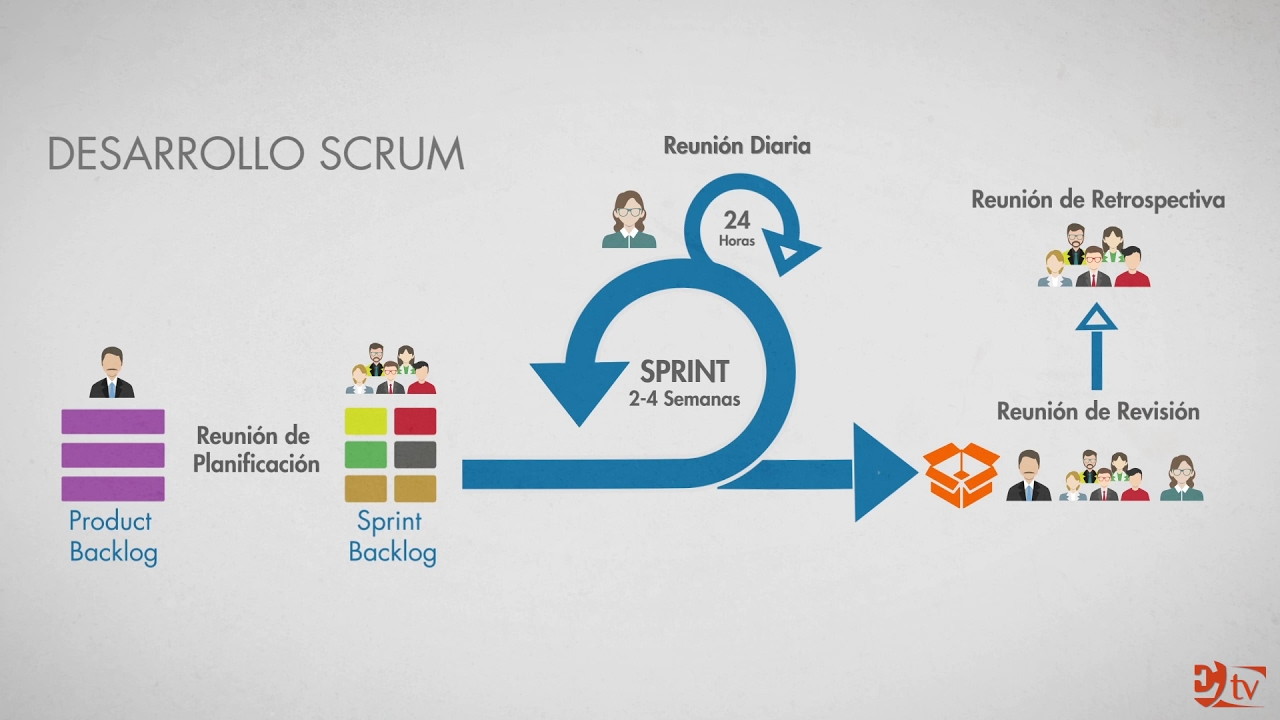
\includegraphics[width=0.8\textwidth]{include/scrumPhases.jpg}
\end{center}

Las fases de Scrum son:
\begin{itemize}
	\item Product backlog: el product owner se encarga de definir los requisitos y diseñar la carga de tareas de los sprints.
	\item Sprint backlog: todo el equipo de Scrum se encarga de crear las historias de usuario conformes a los requisitos. Se balancea la carga de los sprints si es necesario.
	\item Sprint: los desarrolladores empiezan el desarrollo de las tareas. Esta fase suele durar unas dos semanas. Cada día se celebra una reunión que permite al Scrum master y al resto del equipo de desarrolladores cómo va el desarrollo.
	\item Demo: al final del sprint, se realiza una demostración de las funcionalidades cubiertas por el sprint.
	\item Retrospectiva: reunión final del ciclo en la que se reune todo el equipo en la que se evalúa el resultado del sprint, se plantean problemas que hayan ocurrido y se formulan soluciones para la siguiente iteración.
\end{itemize}

Aunque al final no he tenido la ocasión de realizar todas las reuniones pero ha valido la pena este método para ordenar mi trabajo y guardar la información de los requisitos.

\section{Desarrollando en dispositivos móviles (Arquitectura)}
En esta sección se discutirá cómo se ha desarrollado la aplicación y con qué tecnologías se ha llevado a cabo.

El motor está ahora mismo desarrollado para dispositivos móviles de Apple, en el lenguaje de programación Swift \cite{swiftGuides}.

Swift es un lenguaje de programación de propósito general. Fue anunciado en 2014 y es de código abierto. Este proyecto está desarrollado específicamente con la versión 5 de Swift.

Existen muchas formas de programar aplicaciones en Swift: usando arquitecturas nativas como MVC o yendo a ejemplos de arquitecturas limpias como Viper y Clean-Swift.
Sin embargo, debido a que una de las recomendaciones de los pensadores detrás de las arquitecturas limpias es que la arquitectura debe adaptarse a las necesidades del desarrollador, en este proyecto se ha llevado a cabo una mezcla entre estas dos últimas arquitecturas.

\begin{center}
	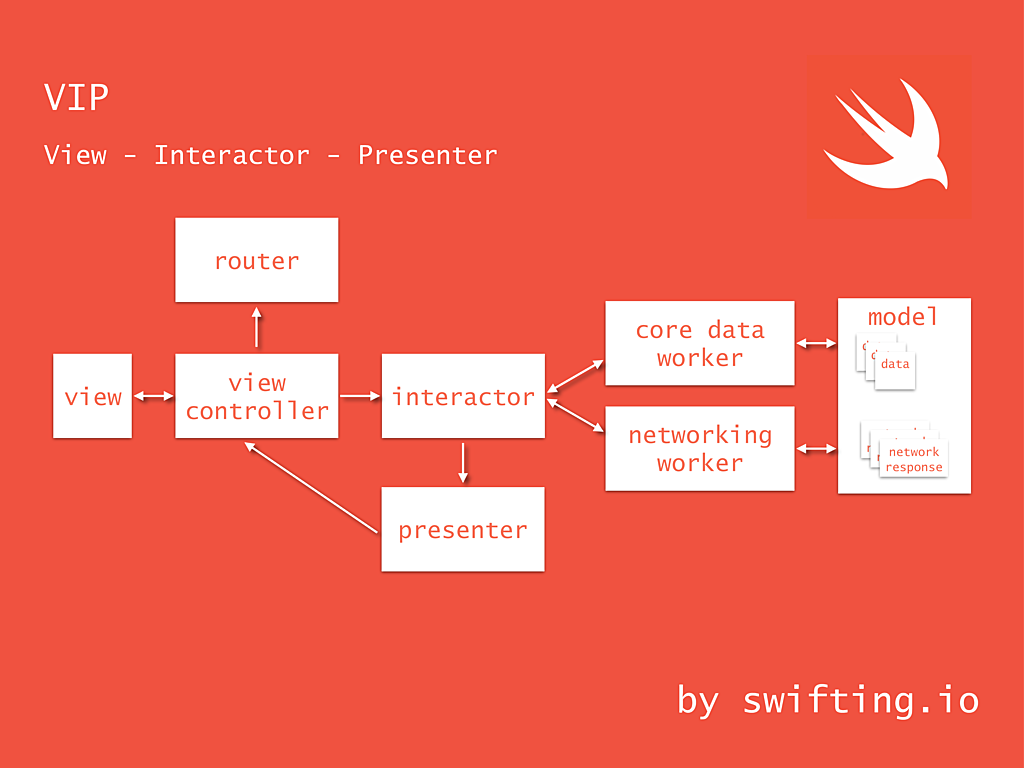
\includegraphics[width=0.75\textwidth]{include/cleanSwiftArchitecture.png}
\end{center}

Para este proyecto se ha planteado desde el principio de su desarrollo una implementación mediante una arquitectura con capas que permita separar elementos de la programación con distintas funcionalidades. Se tomó la decisión de seguir esta arquitectura ya que permite que el código esté modularizado y sea fácil de implementar siguiendo un esquema. En la anterior arquitectura, MVC (Model-View-Controller), se incluía toda la lógica de negocio de la aplicación en los controladores, haciendo muy complicado el mantenimiento del código y la implementación de nuevas funcionalidades.

Proporcionaré el punto de vista de trabajo mediante Xcode el programa especializado en compilar ficheros “swift”.

El proyecto está específicamente dividido en 3 capas.

\subsection{Capa de presentación}
Nivel que se encarga de la interfaz visual que el usuario puede ver y tocar. Esto abarca todos los elementos visuales presentes en la aplicación, como la pantalla de inicio o la pantalla de carga. 
Las vistas se han implementado de esta manera:

\begin{itemize}
	\item \textbf{''Storyboard''}: archivo XML específico de desarrollo en iOS para Objective-C y Swift que recoge toda la información de todos los elementos de una pantalla como pueden ser un botón, la barra de navegación o un deslizador. 
	Incluye todos los elementos que mantienen fija la pantalla, aunque el dispositivo rote o la resolución de la pantalla cambie.
	Estos ficheros se traducen en tiempo real en el entorno de desarrollo, Xcode, para mostrar una vista previa de los elementos en un dispositivo y proporcionar herramientas para ajustar todos los elementos de una vista, todo mediante el llamado ''Interface Builder''.
Este fichero no contiene código en lenguaje Swift en ningún momento.
	\item \textbf{''View Controller''} o controlador de la vista: archivo Swift que incluye información referente a una vista, que puede estar asociada a un ''storyboard'' y que siempre aparece en conjunto con un presentador.
	Este fichero contiene toda la información que conecta lo que se muestra en un dispositivo y las acciones que deben ocurrir al realizar eventos. Tiene una referencia a todos los elementos de una vista, y se encarga de modificarlos.
	En nuestra implementación, los controladores no pueden mantenerse por sí solos, pues solo saben rellenar los datos de los elementos presentes en una vista, como ponerle un nombre a un control o asociar una acción a un botón, pero no saben cómo tienen que rellenar los elementos.
	\item \textbf{''Presenter''} o presentador: archivo Swift que incluye toda la información para rellenar una vista, pero que no tiene acceso a sus elementos. Este fichero tiene siempre asociado un controlador de la vista para saber a cuál tiene que mandarle los datos.
	Contienen toda la información con la que se va a rellenar una vista, como la navegación de una pantalla a otra, el color de los elementos o el lanzamiento de interactores. Suelen contener todas las referencias a los objetos que necesitará una vista para ser rellenada: un enrutador, el controlador al que está asociado, y un protocolo a seguir para que el controlador sepa qué elementos usar de un presentador.
	\item \textbf{''Router''} o enrutador: archivo Swift que incluye toda la información necesaria para navegar a otras vistas en la aplicación, como puede ser ir desde el menú principal a uno secundario. Incluye la referencia al controlador de la vista actual, de manera que le permite cambiarlo por otro durante el transcurso de la aplicación. También es el encargado de crear el presentador y su controlador asociado pertinentes para la nueva vista a mostrar.
\end{itemize}

\subsection{Capa de negocio}
Nivel que se encarga de ejecutar la lógica de negocio de la aplicación. En esta capa se ejecutan todas las acciones que requieren de cierta lógica, como puede ser el cálculo de una operación matemática, el acceso a una base de datos o la utilización de algoritmos complejos.
Esta capa incluye dos tipos de clase principales:
\begin{itemize}
	\item Objetos de dominio: objetos de negocio que se encargan de modelizar todas las posibles estructuras posibles de un objeto en la aplicación. Pongamos el ejemplo de una aplicación de cartas: una carta sería un objeto que representa una instancia de la clase Carta y que contiene toda la información que la define como el palo o el número.
	\item ''Interactor'', o interactores: archivo Swift que incluye una funcionalidad específica para la aplicación. Estos interactores operan con los objetos de dominio y con la capa de datos para ofrecer los resultados de una operación a los presentadores. Una de estas operaciones puede ser sumar dos valores, o recoger información específica de una base de datos.
\end{itemize}

\subsection{Capa de datos}
Nivel que incluye todas las clases con acceso a la base de datos. Estas clases simplemente sirven como puente para la funcionalidad de las librerías propietarias, es decir, desarrolladas por el equipo o de consumo único por la aplicación.
La base de datos que se ha usado en este proyecto es una nativa ofrecida por Apple, Core Data \cite{coreDataDocumentation}.
Esta base de datos permite guardar objetos directamente, sin tener que realizar consultas complicadas. Está basada en una base de datos SQlite.